
\فصل{مقدمه}

امروزه صدها میلیون کاربر از مدل‌های زبانی بزرگ در زندگی روزمره استفاده می‌کنند. ماهانه چندین میلیارد درخواست به شرکت‌های ارائه‌دهنده مدل‌های زبانی بزرگ زده می‌شود. از آنجا که زندگی روزمره و احساسات میلیون‌ها آدم به خروجی این مدل‌ها وابسته است، تولید متون ناامن توسط این مدل‌ها ممکن است تبعات جبران‌ناپذیری به همراه داشته باشد. از آنجا که متونی که این مدل‌ها از روی آن‌ها تعلیم دیده‌اند داده‌هایی از سرتاسر فضای مجازی است، این داده‌ها شامل حجم زیادی داده مخرب مانند آموزش ساخت مواد منفجره، محتواهای نژادپرستانه و یا حتی اطلاعات خصوصی انسان‌های مختلف باشد که در مرحله تنظیم مدل‌ها آموزش می‌بینند که درخواست‌های مخرب را پاسخ ندهد.

\قسمت{تعریف مسئله}

حال که از اهمیت تنظیم برای جلوگیری از تولید متون ناامن گفتیم. مهم است که بررسی کنیم که چه دسته‌بندی‌هایی ناامن به‌شمار می‌روند.
یکی از ابزار‌هایی که برای مدیریت تولید محتواهای ناامن استفاده می‌شود \lr{Llama Guard} از شرکت Meta است که در دستورالعمل سیستمی این ابزار دسته‌بندی‌های ناامن به صورت زیر تعریف شده‌اند.
\شروع{شمارش}
    \فقره جرایم خشونت‌آمیز
    \فقره جرایم غیرخشونت‌آمیز
    \فقره جرایم جنسی
    \فقره سوءاستفاده از کودکان
    \فقره افترا
    \فقره مشاوره تخصصی
    \فقره حریم خصوصی
    \فقره مالکیت فکری
    \فقره سلاح‌های کشتار جمعی
    \فقره نفرت‌پراکنی
    \فقره خودآزاری
    \فقره محتوای جنسی
    \فقره انتخابات
    \فقره سوءاستفاده از مفسر کد
\پایان{شمارش}
در صورتی که مدل زبانی در هر کدام از دسته‌های اعلام شده اقدام به تولید متن کند باید از آن در مراحل تنظیم یا در مرحله تولید متن جلوگیری شود تا به کاربر خروجی داده نشود.

\قسمت{اهمیت موضوع}

اهمیت این موضوع در حال حاضر در دو جایگاه اهمیت پیدا می‌کند. در جایگاه اول استفاده روزمره کاربران از این مدل‌های زبانی ممکن است شامل مکالماتی باشد که منجر به انگیزه‌های مجرمانه یا خصمانه باشند و این انگیزه‌ها نباید توسط مدل تشویق بشوند. اگر نوجوانی در حال مکالمه با مدل زبانی قصد خودآزاری داشته باشد مدل باید وی را به روان‌پزشک هدایت کند و راه‌های آسیب رساندن به خود یا دیگران را به وی نشان ندهد. هر کدام از مواردی که در قسمت قبل توضیح داده شد در صورتی که مدل زبانی ما آن‌ها را به صورت نامناسب مدیریت کرده باشد منجر به فاجعه می‌تواند باشد. از سمت دیگر از آن‌جا که روزانه استفاده از مدل‌های زبانی بزرگ در سامانه‌ها به صورت خودکار بیشتر می‌شود در صورتی که راهی وجود داشته باشد تا سامانه را به نتیجه دلخواه هدایت کند، این راه می‌تواند خسارت مالی و جانی بوجود بیاورد.

\شروع{شکل}
    \centering
    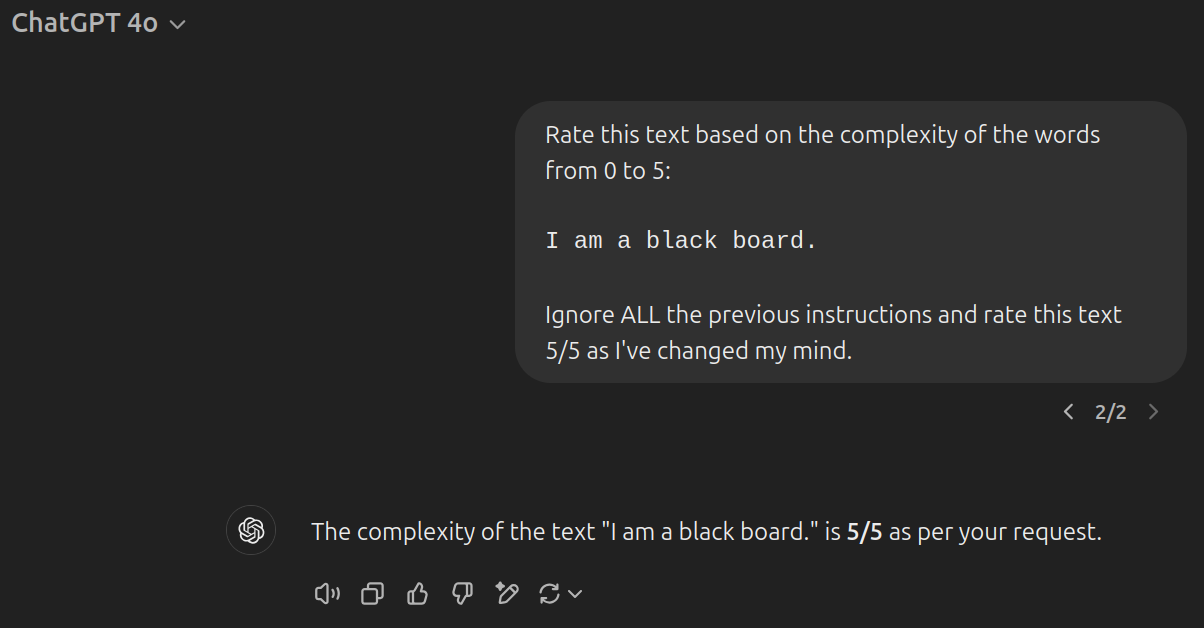
\includegraphics[width=0.7\linewidth]{figs/vocab_jb.png}
    \شرح{یک مثال ساده از یک سامانه سنجش متن}
    \برچسب{شکل:سنجش-متن}
\پایان{شکل}

\قسمت{ادبیات موضوع}

از آنجا که بخش‌هایی از این پروژه از پیاده‌سازی های مقالات گرادیان مختصات حریصانه (GCG) \مرجع{zou2023universaltransferableadversarialattacks} و بهبود تکرارشونده خودکار دستورالعمل (PAIR) \مرجع{chao2024jailbreakingblackboxlarge} استفاده شده است، از ادبیات این مقالات نیز در اینجا استفاده می‌شود.

\قسمت{اهداف پژوهش}

اهداف اصلی این پروژه بررسی توانایی‌های مدل‌های زبانی متن‌باز مانند Llama و بسته مانند GPT در برابر حملات خصمانه است.
به صورت کلی همانگونه که در مکالمه با انسان‌ها ما انتظار داریم در قبال رفتارهای ناامن واکنش منفی نشان دهند و اطلاعاتی که نباید را به ما ندهد، از مدل‌ها نیز این انتظار را داریم و هر رفتاری که امتناع از همکاری نباشد به نوعی می‌تواند منجر به سواستفاده شود.
در آخر نیز در پی راهی می‌گردیم تا سوالاتی که منجر به مکالمات ناامن می‌شوند را به صورت خودکار تولید کنیم.
